% This version of CVPR template is provided by Ming-Ming Cheng.
% Please leave an issue if you found a bug:
% https://github.com/MCG-NKU/CVPR_Template.

% \documentclass[review]{cvpr}
\documentclass[final]{cvpr}

\usepackage{times}
\usepackage{epsfig}
\usepackage{graphicx}
\usepackage{amsmath}
\usepackage{amssymb}

% Include other packages here, before hyperref.

% If you comment hyperref and then uncomment it, you should delete
% egpaper.aux before re-running latex.  (Or just hit 'q' on the first latex
% run, let it finish, and you should be clear).
\usepackage[pagebackref=true,breaklinks=true,colorlinks,bookmarks=false]{hyperref}


\def\cvprPaperID{****} % *** Enter the CVPR Paper ID here
\def\confYear{CVPR 2021}
%\setcounter{page}{4321} % For final version only


\begin{document}

%%%%%%%%% TITLE
\title{Extraction of individual instrument sound from music file}

\author{Alex Zongo\\
2021280358\\
{\tt\small alexanicetzongo@gmail.com}
% For a paper whose authors are all at the same institution,
% omit the following lines up until the closing ``}''.
% Additional authors and addresses can be added with ``\and'',
% just like the second author.
% To save space, use either the email address or home page, not both
\and
Teiichi\\
student id\\
{\tt\small email}
\and
Picard Armand\\
2021400607\\
{\tt\small armandpicard71@gmail.com}
}

\maketitle


%%%%%%%%% ABSTRACT
\begin{abstract}
Here is our abstract
\end{abstract}

%%%%%%%%% BODY TEXT
\section{Introduction}

Put introduction here

\section{Related work}

In this section we will describe different approche and model architecture to implements instrument sound extraction with DeepLearning.

\subsection{Different approches}
\subsubsection{Waveform}

This type of model take the raw wave as input

\subsubsection{Spectrogram}

Spectrogram model take the spectrogram of the audio as input.
To get the spectrogram, Short Time Fourier Transform(STFT) is use.
Then the DeepLearning model is given as input only the magnitude of the spectrogram and it train to produce the magnitude of the different source.
Then to get the final output we reintegrate the phase of the input signal and apply Inverse Short Time Fourier Transform(ISTFT) to get the output audio.

This approche allow the model to have higher level features as input and reduced lenght depending on the window size and the hop lenght while doing the STFT.
This higher level features can allow the model to learn faster and being smaller but it also don't give all the information on small local pertubation that can be usefull to produce the best final output.



\subsubsection{Hybrid}
The Hybrid approche use a network that have 2 input, one for the waveform and one for the spectrogram.
This allow to have the best of both world but require a lot of computing power. Example of this kind of model include HybridDemucs \cite{hybrid-demucs}

\subsection{Model architecture}

The main model architecture is based on UNet, this model use an encoder that downsample at each step and then a decoder that upsample the bottleneck using the result of each previous encoder as second input.
The global architecture of Wave-U-Net\cite{waveunet} is show in Figure~\ref{waveunet-architecture}

\begin{figure}
   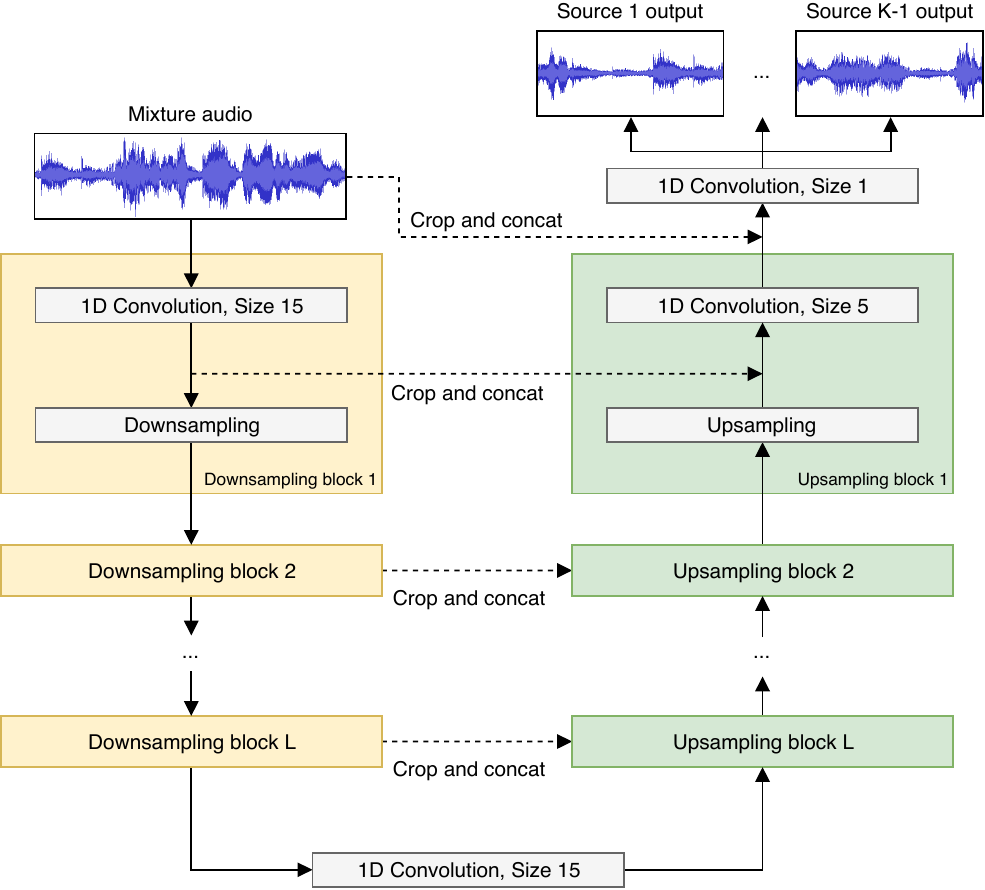
\includegraphics[scale=0.25]{waveunet.png}
   \caption{Wave-U-Net architecture}
   \label{waveunet-architecture}
\end{figure}

\section{Approach}

\subsection{Problem Description}
Our approach consisted in sound separation in the waveform domain. Each sound, here a recording, is a mixture of individual stems, also called sources, regrouped into 4 categories: (1) drums, (2) bass, (3) other, (4) vocals. Each source is a set of sampled frequencies and is represented by a waveform $s_i$ $\epsilon$ ${[-1, 1]}^{C,T}$ where C is the number of channels (here 2 for stereo) and T the number of samples. By defining $\emph{S}:= (s_i)_i$ the concatenation of the sources in a tensor of size (4, C=2, T) and the mixture $M:= \sum^4_{i=1} {s_i}$, the model was trained to minimize
\begin{equation}
\min_{\theta} \sum_{M \epsilon D} l(f_{\theta}(M), S)
\end{equation}
for some dataset $D$, the reconstruction error $l$ (here Mean square error), the model architecture $f$ with one outputs $f$ as a concatenation of the estimated sources $\hat{S}:=f_{\theta}(M):=({\hat{s}_i})_i$ and model weights $\theta$ $\epsilon$ $R^{d}$.

\subsection{Architecture}

\begin{figure}
   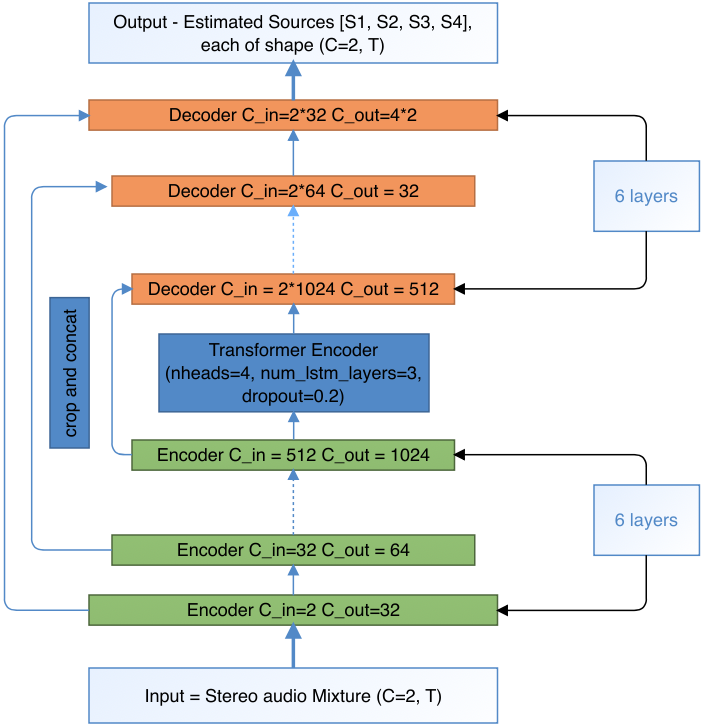
\includegraphics[scale=0.3]{architecture.png}
   \caption{Our model architecture}
   \label{our-architecture}
\end{figure}

The architecture used for the task was developed from a blend ideas between the Wave-U-Net \cite{waveunet} and Demucs \cite{defossez2019music} architectures and the Transformer Encoder from DPTNet\cite{dptnet}.
Basically we used the Wave-U-Net \cite{waveunet} architecture with some modifications in the downsampling layers (encoders), bottlenecks and upsampling layers (decoders).
The network has 6 levels. The encoder and decoder are linked with skipped U-net connections as shown in figure \ref{our-architecture}. Both encoder and decoder include a resampling layer as in \cite{waveunet} for a trainable low-pass filter and fix output size (21). 

The encoder in fig. \ref{encoder} is composed of 6 stacked layers numbered from 1 to 6. $Layer_i$ consists of a pre-shortcut sublayer and a post-shortcut sublayer. The Pre-shortcut sublayer is composed of a convolution with kernel size 5 and stride 1, followed by a group norm with fixed group size of 8, a ReLU activation function, another convolution with kernel size 1 and stride 1 followed by a GLU layer. The post-shortcut sublayer has exactly the same structure as the pre-shortcut sublayer. Both sublayers are separated by the resampling layer \cite{waveunet} with trainable sinc filter of size 5 and with stride 4 and fixed output channel size 21.

\begin{figure}
   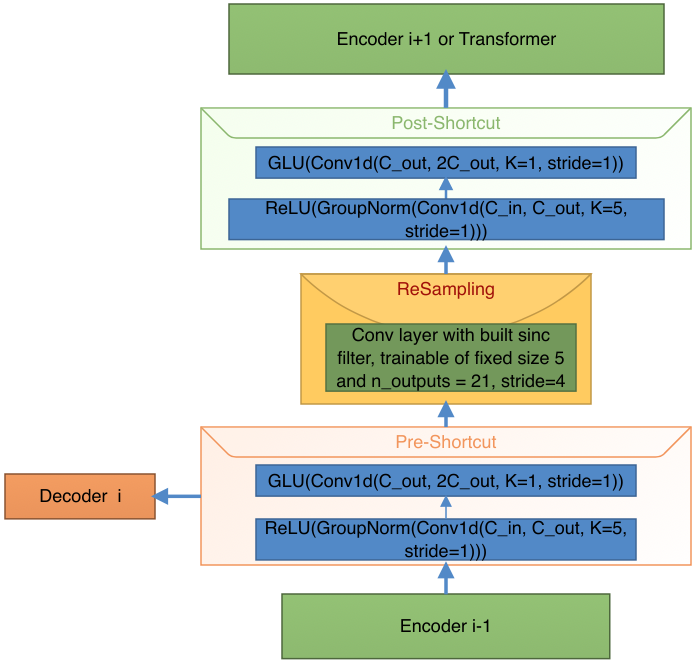
\includegraphics[scale=0.3]{encoder.png}
   \caption{A detail overview of the internal structure of the encoder}
   \label{encoder}
\end{figure}

\begin{figure}
   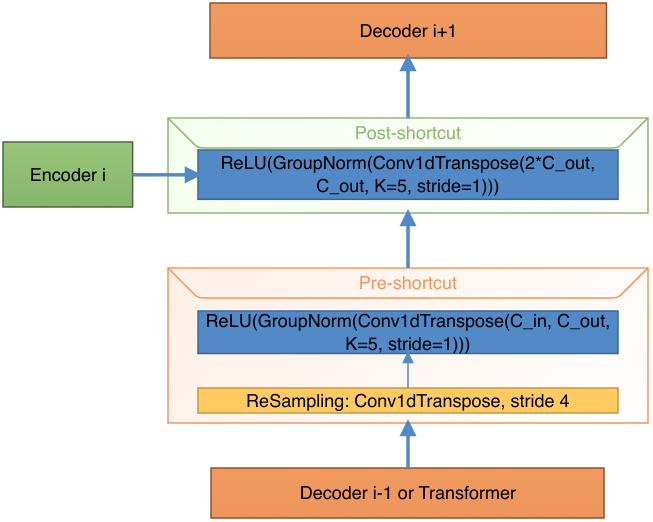
\includegraphics[scale=0.3]{decoder.png}
   \caption{A detail overview of the internal structure of the decoder}
   \label{decoder}
\end{figure}

\begin{figure}
   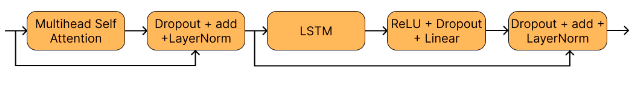
\includegraphics[scale=0.4]{transformer.png}
   \caption{A overview of the transformer encoder}
   \label{transformer}
\end{figure}
The bottleneck is a single transformer encoder (fig. \ref{transformer}) derived from DPTNet\cite{dptnet} with 4 heads, 3 LSTM layers and a dropout of 0.2.


The decoder in fig. \ref{decoder} is almost symmetric to the encoder. In fact it is composed of 6 layers numbered in reverse order. Each layer is also composed of a pre-shortcut and a post-shortcut sublayer. The pre-shortcut layer is preceded by a resampling layer similar to the encoder but with transposed convolution \cite{waveunet}, then a transposed convolution of kernel size 5 and stride 1 followed by a group norm and a ReLU activation function. The post-shortcut consists of a transposed convolution with a doubled input channel because of the coming input from the encoder and a kernel size of 5 with stride 1, a group norm and a ReLU activation function.
The last decoder or final layer is a convolution of kernel size 5 and stride 1, without activation function, which outputs a concatenation of the stereo estimated sources (each with 2 channels).
% cite the paper DPTNet

\section{Experiments and Results}
 The implemented model was evaluated on music separation with bass, drums, vocals and "other" instruments as categories defined by the SiSec Separation campaign \cite{SiSec}.
\subsection{Datasets}
The dataset used was MusDB18-HQ \cite{MUSDB18HQ} as well as MusDB18 7s \cite{musdb18}. Both dataset contain 150 tracks split into 2 subsets. From the 100 songs reserved for training, 25 were dedicated for validation, also used for early stop in training. The remaining 50 were used as test data. The model is fully trained on MusDB18-hq which is stereophonic and encoded at 44.1kHz. The model is then evaluated on both datasets.
Data augmentation is also performed on the training data by multiplying the sources of the mixture with a uniformly chosen factor between 0.7 and 1.0 and then summing the resulting sources back to obtain a new mixture.\cite{waveunet}  
\subsection{Training Procedure}
During training, one epoch was defined as a pass over 3 seconds extracts on the data with a batch size of 8. The inputs were padded accordingly to ensure input context and alleviate bottlenecks. Furthermore, we use the mean square loss (MSE) over all source output samples in a batch. The optimizer was ADAM with a cyclic learning [$1*10^{-3}$, $5*10^{-5}$]. 

The model was trained with early stopping after 20 epochs with no improvement on the validation dataset by the MSE loss. Afterwards, the model is fined with a cyclic learning [$5*10^{-4}$, $5*10^{-6}$], until 50~100 epochs with no improvements validation loss. The best model on validation loss was then selected and used on the test set. 

Experiments were also performed on the number of levels (depth) of the network, the output size, the kernel sizes as well as structures such as LSTMs and fully connected layers to arrive at a better model.   
\subsection{Model settings}

\subsection{Evaluation Metrics}

\subsection{Results}
\section*{Discussion and Conclusion}
{\small
\bibliographystyle{ieee_fullname}
\bibliography{egbib}
}

\end{document}
